\documentclass[12pt, a4paper]{article}

% -------------------------------------------------------------------
% PACKAGES
% -------------------------------------------------------------------
\usepackage[utf8]{inputenc}
\usepackage{graphicx}
\usepackage{geometry}
\usepackage{hyperref}
\usepackage{listings}
\usepackage{xcolor}
\usepackage{booktabs}
\usepackage{float}
\usepackage{caption}
\usepackage{amsmath}
\usepackage{subcaption}

% -------------------------------------------------------------------
% PAGE SETUP
% -------------------------------------------------------------------
\geometry{margin=2.5cm}
\setlength{\parskip}{1em}
\setlength{\parindent}{0pt}

% -------------------------------------------------------------------
% CODE STYLING
% -------------------------------------------------------------------
\definecolor{codegreen}{rgb}{0,0.6,0}
\definecolor{codegray}{rgb}{0.5,0.5,0.5}
\definecolor{codepurple}{rgb}{0.58,0,0.82}
\definecolor{backcolour}{rgb}{0.97,0.97,0.97}

\lstdefinestyle{mystyle}{
    backgroundcolor=\color{backcolour},
    commentstyle=\color{codegreen},
    keywordstyle=\color{magenta},
    numberstyle=\tiny\color{codegray},
    stringstyle=\color{codepurple},
    basicstyle=\ttfamily\footnotesize,
    breakatwhitespace=false,
    breaklines=true,
    captionpos=b,
    keepspaces=true,
    numbers=left,
    numbersep=5pt,
    showspaces=false,
    showstringspaces=false,
    showtabs=false,
    tabsize=4,
    frame=single
}
\lstset{style=mystyle}

% -------------------------------------------------------------------
% METADATA
% -------------------------------------------------------------------
\title{
    \textbf{CSY3058 Media Technology: Assessment 1}\\
    \large Design, Implementation, and Critical Evaluation of a Smart Security Camera System\\
    \large \textit{Scenario: Northampton Warehouse Facility}
}
\author{Ryan Gichuru \; Student ID: 22837352}
\date{\today}

\begin{document}

\maketitle

% -------------------------------------------------------------------
% ABSTRACT
% -------------------------------------------------------------------
\begin{abstract}
\textbf{Summary:} This report documents the design and evaluation of a Python-based smart security camera pipeline for a warehouse environment. The implementation intentionally uses a \textit{pure-Python + OpenCV} architecture (no cloud services, no managed inference) to demonstrate what a ``baseline'' CCTV analytics system looks like when engineered from first principles. The system uses a two-stage approach: (1) background subtraction (MOG2) as a low-cost motion gate, followed by (2) person verification using either a classical HOG (Histogram of Oriented Gradients) people detector or a lightweight deep model (MobileNet-SSD via OpenCV DNN). A probabilistic presence tracker based on log-odds updates is used to stabilise detections over time.

Evaluation on the WiseNET CCTV dataset (manual human annotations as ground truth) shows that the deep model produces substantially better localisation than HOG (Mean IoU $0.5065$ vs $0.3560$ on the expanded split), while both pipelines remain conservative on recall ($\approx 0.33$) due to upstream motion gating choices. Dataset-provided YOLOv3/SSD-512 models outperform the lightweight approaches on recall and IoU, supporting the recommendation that YOLO-class detectors are preferred for deployment when hardware permits.
\end{abstract}

\tableofcontents
\newpage

% -------------------------------------------------------------------
% SECTION 1: INTRODUCTION
% -------------------------------------------------------------------
\section{Introduction}
\label{sec:intro}

\subsection{Project Scenario and Objectives}
This project addresses the security requirements of a large warehouse facility in Northampton. The system aims to reduce reliance on manual guard patrols by monitoring a fixed CCTV feed and producing actionable evidence clips when a breach is likely.

The primary objectives are:
\begin{itemize}
    \item \textbf{Detect motion} robustly in a static camera feed while tolerating noise (compression artefacts, exposure changes, shadows).
    \item \textbf{Verify people} and suppress non-human motion using computer vision.
    \item \textbf{Archive evidence} by recording incident clips with overlays and metadata.
    \item \textbf{Minimise false alarms} (high precision) to avoid alert fatigue.
\end{itemize}

\subsection{Media Technology Context (Why This Problem Is Hard)}
A warehouse CCTV feed is a multimedia signal with properties that directly affect detection reliability:
\begin{itemize}
    \item \textbf{Frame sampling:} CCTV streams are typically 25--30 fps. Motion detection quality depends on temporal sampling and how fast the background model adapts.
    \item \textbf{Compression artefacts:} block noise and temporal prediction errors can create spurious foreground blobs that must be removed with morphology and temporal gating.
    \item \textbf{Illumination dynamics:} automatic exposure, shadows, and reflections create non-object ``motion'' that classical frame differencing cannot reliably ignore.
\end{itemize}

Because of these constraints, the system is designed as a staged pipeline where cheap operations filter most frames before expensive inference.

\subsection{Why a ``Pure Python'' Baseline Architecture}
The system is deliberately implemented as a \textit{local, pure-Python pipeline} (OpenCV + NumPy + PySide6) to:
\begin{itemize}
    \item demonstrate end-to-end engineering (video I/O, processing, recording, UI) without managed services,
    \item expose how parameter choices (thresholds, morphology, temporal gating) impact detection in CCTV media,
    \item provide a reference baseline before recommending stronger deployment-grade detectors.
\end{itemize}

\subsection{Report Structure}
This report outlines: (1) design foundations (motion gating and person verification), (2) implementation details (core modules in \texttt{src/ssc/}), (3) evaluation methodology and results on WiseNET, and (4) critical discussion including strengths, weaknesses, and deployment recommendations.

\subsection{Terminology and Definitions}
For clarity, the report uses the following terms consistently:
\begin{itemize}
    \item \textbf{Ground truth (GT):} the reference label used for evaluation. In this report, \textbf{manual GT} refers to the dataset's human-annotated bounding boxes.
    \item \textbf{Presence detection:} a frame-level decision of whether a person is present (with or without a usable bounding box).
    \item \textbf{Localisation:} how accurately the predicted bounding box overlaps the GT box, measured by IoU.
    \item \textbf{Motion gate / stability gate:} the upstream decision that motion is present and persistent enough (over $N$ frames) to warrant downstream verification.
    \item \textbf{ROI:} regions of interest (rectangles) limiting where detections are accepted.
    \item \textbf{TP/FP/FN/TN:} true/false positives/negatives for frame-level presence.
\end{itemize}

\subsection{AI-Assisted Work (Disclosure)}
This project utilises AI assistance for accelerating development and documentation. Specifically:
\begin{itemize}
    \item \textbf{Code Generation:} Utility scripts (e.g., runtime benchmarking) and the log-odds update logic in the probability tracker were drafted with AI assistance (GPT-4 concept generation), then verified and tuned manually.
    \item \textbf{Report Writing:} Sections of this report were drafted using AI tools to summarise technical details and format LaTeX, then reviewed and refined by the author to ensure accuracy and alignment with the implemented system.
\end{itemize}
All evaluation outputs, metrics, and figures presented in this report are generated by the actual submitted code running on the specific dataset splits.

% -------------------------------------------------------------------
% SECTION 2: LITERATURE REVIEW
% -------------------------------------------------------------------
\section{Literature Review}
\label{sec:lit_review}

The surveillance industry has undergone a paradigm shift from passive recording to active intelligence. This section reviews the evolution of video surveillance technologies and compares the algorithmic approaches relevant to this project.

\subsection{Evolution of Video Surveillance Systems}
Early surveillance systems (Classic CCTV) were purely analog, relying on VCR tapes and constant human monitoring. These ''Generation 1`` systems suffered from limited storage and the inability to trigger automatic alerts \cite{velastin2006}. The transition to digital (Generation 2) introduced DVRs and IP cameras, enabling higher resolutions, network transmission, and basic motion detection based on pixel differences \cite{valera2005}.

Modern systems (Generation 3/Smart Surveillance) integrate Artificial Intelligence (AI) to analyse video content in real-time. Unlike basic motion detection, which triggers on any pixel change (including shadows or swaying trees), intelligent systems use Computer Vision to classify objects (person vs. vehicle) and understand behaviour \cite{briefcam2020}. This shift aims to solve the ''data deluge`` problem, where security operators are overwhelmed by thousands of hours of irrelevant footage.

\subsection{Motion Detection Techniques}
\textbf{Background Subtraction (BGS):} Traditional techniques like Gaussian Mixture Models (MOG2) model the background as a probability distribution per pixel. This allows them to adapt to gradual lighting changes while isolating moving foreground objects \cite{zivkovic2004mog2}. MOG2 is computationally efficient ($\approx 200+$ FPS on CPU) but prone to false positives from sudden lighting shifts or environmental noise.

\textbf{Deep Learning Object Detection:} Contemporary research favours Convolutional Neural Networks (CNNs) for robustness. Detectors like YOLO (You Only Look Once) and SSD (Single Shot Detector) learn rich feature representations, allowing them to detect people even in complex clutter where BGS fails \cite{redmon2016yolo}. However, these models require significantly more compute power, creating a trade-off between accuracy and latency on edge devices.

\subsection{Probabilistic Tracking in Surveillance}
Raw detections can be jittery or intermittent. To address this, surveillance systems often employ tracking filters. Classic approaches use Kalman Filters to predict object state \cite{bewley2016simple}. More simplified approaches for presence detection use Bayesian filters or occupancy grids (log-odds), which act as a temporal low-pass filter, accumulating confidence over detection sequences to smooth out momentary detector failures \cite{thrun2005probabilistic}.

\subsection{Context of This Project}
This project allows for a comparative study by implementing a hybrid architecture: using traditional BGS for high-speed gating and modern Deep Learning (MobileNet-SSD) for verification, effectively bridging the gap between Generation 2 efficiency and Generation 3 intelligence.

% -------------------------------------------------------------------
% SECTION 3: DESIGN AND THEORETICAL FOUNDATION
% -------------------------------------------------------------------
\section{Design and Theoretical Foundation}
\label{sec:design}

\subsection{Pipeline Overview}
The pipeline is multi-stage:
\begin{enumerate}
    \item \textbf{Video ingest:} frames are read from a file using OpenCV.
    \item \textbf{Motion gate:} MOG2 background subtraction + morphology generates foreground blobs.
    \item \textbf{Stability gate:} motion must persist for $N$ frames before triggering, and must be absent for $M$ frames before clearing.
    \item \textbf{Person verification:} when motion is stable, run a person detector (HOG or DNN) on ROI(s).
    \item \textbf{Recorder:} incident clips and metadata are written once an incident is active.
\end{enumerate}

This design is aligned with real-time constraints: run expensive models only when motion indicates the possibility of a meaningful event.

\subsection{Motion Detection via MOG2 Background Subtraction}
Running deep models continuously on a 24/7 feed is computationally expensive. Background subtraction acts as a low-cost filter.

We use OpenCV's MOG2 algorithm (Gaussian mixture model per pixel) which adapts to gradual illumination changes while segmenting sudden foreground motion \cite{zivkovic2004mog2,opencv_mog2}. MOG2 is preferable to simple differencing because it maintains a statistical model of the background distribution.

\subsection{Mask Cleaning and Morphology}
Foreground masks are noisy due to compression artefacts and shadow segmentation. Morphological opening/closing and dilation are used to:
\begin{itemize}
    \item remove small speckles (opening),
    \item fill holes in blobs (closing),
    \item connect fragmented body parts into coherent contours (dilation).
\end{itemize}
These operations are standard tools in image processing pipelines \cite{opencv_morph}.

\subsection{Person Verification: Classical HOG (Why Start Here?)}
Before integrating deep learning, the system implements a classical computer vision baseline using \textbf{Histogram of Oriented Gradients (HOG)}.

\begin{enumerate}
    \item \textbf{HOG Approach:} This uses OpenCV's default people detector (linear SVM on HOG features). It operates by computing gradient orientations in local grid cells and normalizing them over blocks \cite{dalal2005hog}.
    \item \textbf{Why HOG First:} It provides an explainable, low-resource baseline. It does not require a GPU or heavy model weights, making it a suitable starting point for "edge" verification. However, it is sensitive to occlusion and non-upright poses.
\end{enumerate}

\subsection{Deep Learning Integration (MobileNet-SSD and Options)}
To address the limitations of HOG, the system integrates Deep Learning options using OpenCV's DNN module.

\begin{enumerate}
    \item \textbf{MobileNet-SSD (Primary DL Model):} The system uses a MobileNet backbone with an Single Shot Detector (SSD) head. This offers a balance of speed and accuracy suitable for CPU inference \cite{liu2016ssd,howard2017mobilenets}.
    \item \textbf{YOLO Option (Available Extension):} The WiseNET dataset provides baselines from heavier models like YOLOv3. In this project, YOLO is implemented as an \textit{available option} (via Ultralytics) to demonstrate how a stronger model can plug into the same pipeline. While not the primary focus of the minimal "pure-Python" submission, it is available for testing when higher recall is required \cite{redmon2018yolov3}.
\end{enumerate}

% -------------------------------------------------------------------
% SECTION 3: IMPLEMENTATION
% -------------------------------------------------------------------
\section{Implementation}
\label{sec:implementation}

The solution is implemented in Python 3.x using OpenCV for video I/O, background subtraction, drawing, and DNN inference. The core processing pipeline is in \texttt{src/ssc/pipeline.py}; motion detection is in \texttt{src/ssc/motion.py}; probabilistic smoothing is in \texttt{src/ssc/features/probabilistic\_presence.py}; and the interactive UI is in \texttt{src/ssc/qt\_gui.py}.

\subsection{Interactive GUI Implementation (Media Control in Practice)}
A PySide6 (Qt) application supports parameter tuning and live preview. This aligns with multimedia engineering practice: thresholds and temporal filters must often be calibrated per camera due to lens, lighting, and compression differences.

The GUI also allows the ROI to be set either by drawing rectangles directly on the preview or by selecting an automatic full-frame ROI mode for quick testing.

\begin{figure}[H]
    \centering
    % NOTE: The screenshot is optional for compilation; if absent, a placeholder box is rendered.
    \IfFileExists{Images/gui_screenshot.png}{
        \includegraphics[width=0.85\linewidth]{Images/gui_screenshot.png}
    }{
        \fbox{\parbox{0.85\linewidth}{\centering GUI screenshot not found (expected: \texttt{Images/gui\_screenshot.png}).}}
    }
    \caption{Security Camera Qt GUI allowing real-time parameter tuning and preview.}
    \label{fig:gui}
\end{figure}



\subsection{Motion Gating and Temporal Stability}
In \texttt{src/ssc/motion.py}, MOG2 produces a foreground mask which is filtered by thresholding and morphology. In \texttt{src/ssc/pipeline.py}, stability is enforced using \texttt{motion\_on\_frames} and \texttt{motion\_off\_frames}:
\begin{itemize}
    \item \textbf{On-gate ($N$ frames):} requires consecutive frames of motion to trigger.
    \item \textbf{Off-gate ($M$ frames):} requires consecutive non-motion frames to clear.
\end{itemize}
This reduces one-frame artefacts typical of compressed CCTV video.

\begin{lstlisting}[language=Python, caption=Motion Detection Initialisation (src/ssc/motion.py)]
class MotionDetector:
    def __init__(self, cfg: MotionConfig):
        self._subtractor = cv2.createBackgroundSubtractorMOG2(
            history=cfg.mog2_history,
            varThreshold=cfg.mog2_var_threshold,
            detectShadows=cfg.mog2_detect_shadows,
        )
        self._kernel = cv2.getStructuringElement(
            cv2.MORPH_ELLIPSE, (cfg.morph_kernel, cfg.morph_kernel)
        )
\end{lstlisting}

\subsection{HOG Person Detection (Classical Baseline)}
The HOG pipeline uses OpenCV's default people detector (linear SVM on HOG features). It is used as a baseline for explainable, low-cost verification and is sensitive to pose, scale, and occlusion, which is why it is positioned before the deep learning options.

We do not include a full HOG tuning guide here; in testing, the best-performing configuration was the default settings currently used in the pipeline, so further parameter tweaks did not materially improve results.

\subsection{Deep Learning Integration (OpenCV DNN + YOLO Option)}
When motion is stable, the pipeline can run MobileNet-SSD. Frames are pre-processed using \texttt{blobFromImage} with scaling $1/127.5$ and mean subtraction 127.5, mapping pixel intensities to $[-1, 1]$.

\begin{lstlisting}[language=Python, caption=DNN Pre-processing (src/ssc/features/dnn_person_detector.py)]
h, w = frame_bgr.shape[:2]
blob = cv2.dnn.blobFromImage(frame_bgr, 0.007843, (300, 300), 127.5)
net.setInput(blob)
detections = net.forward()
\end{lstlisting}

YOLO is available as an optional deep learning detector (Ultralytics) with class filtering and rate-limited inference to keep CPU workloads manageable.

\subsection{Probabilistic Presence Tracker (Intelligence Layer)}
The motion gate is deliberately conservative to avoid false alarms, but this also risks intermittent ``misses'' due to occlusion or detector jitter. To mitigate this, an intelligence layer models presence probabilistically rather than as a hard binary.

The tracker uses a log-odds representation $l_t = \log\frac{p_t}{1-p_t}$, similar to occupancy-grid and Bayes filter approaches \cite{thrun2005probabilistic}. The update is:
\begin{align}
    l_t &= l_{t-1} + \log\frac{p(z_t\mid \text{present})}{1-p(z_t\mid \text{present})} - \log\frac{p_0}{1-p_0}
\end{align}
where $p_0$ is the prior (initial belief). In implementation, detections push $l_t$ upward; misses decay it using two miss rates (a gentle decay when already confident, and a stronger decay when not).

\begin{lstlisting}[language=Python, caption=Probabilistic Presence Update (src/ssc/features/probabilistic_presence.py)]
if detected_bbox is not None:
    self._state.log_odds += self._logit(self.cfg.p_det) - self._prior_log_odds
    self._state.bbox = self._ema_bbox(self._state.bbox, detected_bbox)
else:
    miss_p = self.cfg.p_miss_strong if self._state.probability >= self.cfg.p_show else self.cfg.p_miss
    self._state.log_odds += self._logit(miss_p) - self._prior_log_odds
\end{lstlisting}

This mechanism provides temporal smoothing (stability) while still reacting to sustained absence. New improvements allow the UI to decouple these functions: the operator can enable smoothing (logic) independently of the confidence display (overlay), reducing visual clutter while maintaining tracking stability.

\subsubsection{Core Logic Implementation}
The core logic for this probabilistic update is implemented in \texttt{src/ssc/features/probabilistic\_presence.py}. It balances the detector confidence against a decay factor.

\begin{lstlisting}[language=Python, caption=Probabilistic Presence Update Logic]
def update(self, detected_bbox, in_roi=True):
    if detected_bbox is not None:
        # Increase belief (Log-Odds)
        self._state.log_odds += self._logit(self.cfg.p_det) - self._prior_log_odds
        self._state.bbox = self._ema_bbox(self._state.bbox, detected_bbox)
    else:
        # Decay belief
        # Use stronger decay if we were already confident (reduces ghosting)
        miss_p = self.cfg.p_miss_strong if self._state.probability >= self.cfg.p_show else self.cfg.p_miss
        self._state.log_odds += self._logit(miss_p) - self._prior_log_odds
        
    # Clamp to avoid saturation
    self._state.log_odds = _clamp(
        self._state.log_odds, 
        self.cfg.log_odds_min, 
        self.cfg.log_odds_max
    )
\end{lstlisting}

This logic ensures that a single missed detection frame does not immediately drop the track, but sustained absence will eventually clear it.

In practice, this ``intelligence engine'' is a compensating layer for the weaknesses of the HOG pipeline: it does not fix HOG localisation, but it reduces flicker and stabilises evidence clips.

% -------------------------------------------------------------------
% SECTION 4: EVALUATION AND RESULTS
% -------------------------------------------------------------------
\section{Evaluation and Results}
\label{sec:eval}

\subsection{Dataset and Ground Truth}
Evaluation uses the WiseNET CCTV dataset. Throughout this report, \textbf{ground truth (GT)} refers to the dataset's \textbf{manual human annotations}. Dataset-provided automatic detector outputs (YOLOv3/SSD-512) are treated as additional reference baselines, not as GT \cite{wisenet_readme}.

WiseNET is used here only for \textbf{testing and evaluation} of the implemented pipeline; no model training is performed as part of this submission.

Two splits are used:
\begin{itemize}
    \item \textbf{Expanded split:} \texttt{data/wisenet\_split.json} (18 videos across sets 1,2,3,4,5,9,11).
    \item \textbf{Option A split:} \texttt{data/wisenet\_split\_option\_a.json} (8 videos; balanced snapshot).
\end{itemize}

\subsection{Metrics}
We report:
\begin{itemize}
    \item \textbf{Frame-level Precision/Recall/F1} for presence detection.
    \item \textbf{IoU} (Intersection over Union) for localisation where both GT and prediction contain boxes.
    \item \textbf{Temporal latency (frames)} for entry/exit timing.
    \item \textbf{Person continuity} (max correct streak and continuity rate while GT is present).
    \item \textbf{Probability alignment} (mean presence probability on GT-present vs GT-absent frames when probability output is enabled).
\end{itemize}

\subsection{HOG Integrity Sanity Check (Correctness, Not Performance)}
Before interpreting HOG underperformance as a modelling limitation, a basic integrity check is performed to reduce the risk of evaluation artefacts:
\begin{itemize}
    \item \textbf{Descriptor dimensionality check:} confirm OpenCV HOG feature vectors match the expected descriptor length for the configured window.
    \item \textbf{Qualitative check:} compute a HOG visualisation and confirm highlighted gradients align with the observed silhouette in representative frames.
\end{itemize}

This sanity check does not claim accuracy; it supports that poor results are not caused by a broken feature extraction pipeline.

\subsection{Per-Video Robustness (Failure Modes and Variability)}
Aggregate metrics can hide strong variation across clips (camera angle, illumination changes, compression, and whether the clip contains people). To show robustness and failure modes, Table \ref{tab:per_video_extremes} summarises best/worst cases on the expanded split.

\begin{table}[H]
\centering
\caption{Per-video extremes (expanded split, manual GT). The frame-level presence metrics are identical for our HOG and DNN pipelines on this split because both use the same upstream motion+stability gate; the key difference is localisation quality (IoU).}
\label{tab:per_video_extremes}
\begin{tabular}{llr}
\toprule
Metric & Video (example) & Value \\
\midrule
Best frame-level F1 & set\_11/video11\_3.avi & 0.915 \\
Best frame-level F1 & set\_11/video11\_1.avi & 0.868 \\
Best frame-level F1 & set\_5/video5\_3.avi & 0.838 \\
\addlinespace
Worst frame-level F1 & set\_9/video9\_1.avi & 0.000 \\
Worst frame-level F1 & set\_9/video9\_2.avi & 0.000 \\
Worst frame-level F1 & set\_9/video9\_3.avi & 0.000 \\
\addlinespace
Best IoU (DNN) & set\_5/video5\_3.avi & 0.751 \\
Best IoU (DNN) & set\_11/video11\_3.avi & 0.743 \\
Best IoU (DNN) & set\_4/video4\_1.avi & 0.672 \\
\addlinespace
Best IoU (HOG) & set\_4/video4\_1.avi & 0.468 \\
Best IoU (HOG) & set\_5/video5\_3.avi & 0.466 \\
Best IoU (HOG) & set\_11/video11\_3.avi & 0.441 \\
\bottomrule
\end{tabular}
\end{table}

\subsection{Confusion Matrix View (Frame-Level Presence)}
For the expanded split vs manual ground truth, the aggregate confusion counts are (TP, FP, FN, TN) = (5689, 528, 11685, 18011) for both HOG and DNN presence detection, reflecting that the motion gate dominates which frames are eligible for downstream verification.

\begin{table}[H]
\centering
\caption{Frame-level presence confusion matrix (expanded split, manual GT; our pipelines).}
\label{tab:confusion_presence}
\begin{tabular}{lrr}
\toprule
 & Predicted Present & Predicted Absent \\
\midrule
GT Present & TP = 5689 & FN = 11685 \\
GT Absent & FP = 528 & TN = 18011 \\
\bottomrule
\end{tabular}
\end{table}

\subsection{Runtime (Throughput on CPU)}
To evidence feasibility as a media-processing service, we measured runtime throughput (FPS) using a small benchmark script (\texttt{tools/benchmark\_runtime.py}). \textit{Note: this script was generated with assistance to speed up benchmarking and ensure repeatability.}

The benchmark measures \textbf{decode + motion gate + optional person model} and intentionally avoids recorder/overlay I/O. Measurements were taken on Windows 10 (Python 3.10.11, OpenCV 4.13.0; 32 logical CPU cores). Each run processes 600 frames and excludes an initial warmup of 30 frames to reduce one-off model-load noise. Two representative clips were used:
\begin{itemize}
    \item \textbf{video4\_1.avi (set\_4):} person-present footage (more stable motion, more model invocations).
    \item \textbf{video9\_1.avi (set\_9):} no-person footage (model invocations occur only on occasional false motion).
\end{itemize}

\begin{table}[H]
\centering
\caption{Runtime benchmark results (average FPS and model-call cost). ``Calls/100f'' indicates how often the person model ran due to motion+stability gating and the detector interval. YOLO is marked N/A here because Ultralytics was not installed in the benchmark environment at measurement time.}
\label{tab:runtime_benchmark}
\begin{tabular}{lrrrrrr}
\toprule
Backend & FPS (video4\_1) & Calls/100f & Avg call ms & FPS (video9\_1) & Calls/100f & Avg call ms \\
\midrule
Motion gate only & 213.86 & 0.00 & -- & 489.34 & 0.00 & -- \\
HOG verification & 88.58 & 10.33 & 64.55 & 605.44 & 1.17 & 14.54 \\
DNN verification & 204.68 & 6.17 & 12.80 & 609.11 & 0.83 & 22.12 \\
YOLO verification & N/A & N/A & N/A & N/A & N/A & N/A \\
\bottomrule
\end{tabular}
\end{table}

\textbf{Interpretation:} the DNN backend has a substantially lower per-invocation cost than HOG on this hardware, and because person verification is rate-limited (and in practice often gated by stable motion), overall throughput remains high when motion is absent. This is consistent with the design goal: minimise expensive inference unless the media signal indicates a plausible event.

\subsection{Core Result: HOG vs DNN (Manual GT, Expanded Split)}
Table \ref{tab:manual_expanded} summarises the main finding: \textit{DNN localisation is substantially better than HOG}, even when frame-level P/R is identical due to upstream gating.

\begin{table}[H]
\centering
\caption{Aggregate results vs manual annotations (expanded split). Values taken from project evaluation outputs (\texttt{evaluations/metrics/metrics\_*.json}) and summarised in \texttt{docs/project/EVALUATION\_REPORT.md}.}
\label{tab:manual_expanded}
\begin{tabular}{lrrrr}
\toprule
Model & Precision & Recall & F1 & Mean IoU \\
\midrule
Our HOG & 0.9151 & 0.3274 & 0.4823 & 0.3560 \\
Our DNN (MobileNet-SSD) & 0.9151 & 0.3274 & 0.4823 & 0.5065 \\
Auto SSD\_512 & 0.9973 & 0.7646 & 0.8656 & 0.7187 \\
Auto YOLOv3\_608 & 0.9974 & 0.7062 & 0.8269 & 0.7336 \\
\bottomrule
\end{tabular}
\end{table}

\textbf{Interpretation:} HOG produces weaker bounding boxes and misses more positives. The MobileNet-SSD DNN improves localisation (IoU), which is operationally important for evidence overlays and downstream tracking. However, both ``Our'' pipelines have limited recall due to motion gating and conservative stability thresholds.

These outcomes are visualised in the summary plots (presence P/R/F1 and IoU comparison) and are the primary evidence for the conclusion that HOG performs poorest on localisation while YOLO/SSD remain stronger on both recall and IoU.

\begin{figure}[H]
    \centering
    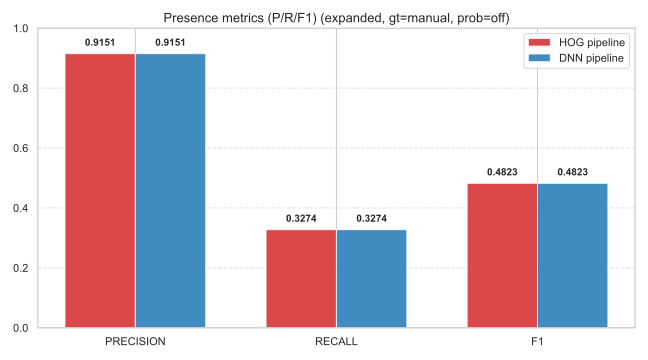
\includegraphics[width=0.75\linewidth]{Images/prf1_expanded_manual_prob_off.png}
    \caption{Frame-level presence Precision/Recall/F1 (expanded split, manual GT; probability off).}
    \label{fig:prf1_expanded}
\end{figure}

\begin{figure}[H]
    \centering
    \includegraphics[width=0.80\linewidth]{Images/iou_comparison_expanded_manual_prob_off.png}
    \caption{Localisation IoU comparison (expanded split, manual GT; probability off).}
    \label{fig:iou_comparison_expanded}
\end{figure}

\subsection{Class Balance and Precision Inflation}
Warehouse CCTV contains long periods with no people. This inflates precision for conservative models because the negative class dominates. The project computed class balance over the split (\texttt{evaluations/class\_balance.json}).

\begin{figure}[H]
    \centering
    % USER ACTION: generated by evaluation notebook/scripts and placed in Images/
    \includegraphics[width=0.6\linewidth]{Images/class_balance_expanded.png}
    \caption{Class balance (expanded split), showing high prevalence of negative frames.}
    \label{fig:balance}
\end{figure}

\subsection{Latency: Early Warning Effect}
The pipeline exhibits negative entry latency (early trigger). This occurs because MOG2 responds to environmental changes (door opening, cast shadows) before the person is fully visible, producing an ``early warning'' effect.

\begin{figure}[H]
    \centering
    \includegraphics[width=0.7\linewidth]{Images/latency_expanded_manual_prob_off.png}
    \caption{Latency distribution (negative indicates early detection).}
    \label{fig:latency}
\end{figure}

\subsection{Qualitative Error Analysis (False Positives / False Negatives)}
The per-video breakdown highlights failure modes that map directly to pipeline stages:
\begin{itemize}
    \item \textbf{False positives in ``no-person'' clips:} several video9\_* clips have GT present = 0 but non-zero FP. This typically occurs when the background model and morphology produce foreground blobs (e.g., illumination/exposure shifts, shadows, or compression artefacts), causing the motion gate to trigger even though no person is present.
    \item \textbf{False negatives dominated by gating:} clips with long or subtle motion can fail to meet stability thresholds, leading to high FN even if the downstream detector is capable. This is consistent with identical frame-level P/R for HOG and DNN on the expanded split.
    \item \textbf{Localisation failures:} when motion is correctly gated, HOG often produces weaker bounding boxes than DNN due to pose/scale sensitivity, reducing IoU even when presence is correctly detected.
\end{itemize}

\begin{figure}[H]
    \centering
    \includegraphics[width=0.90\linewidth]{Images/presence_timeline_video4_1_hog.png}
    \caption{Example presence timeline (video4\_1) illustrating temporal behaviour and errors across frames.}
    \label{fig:presence_timeline_example}
\end{figure}

\subsection{Probability vs. Actual Events}
A key evaluation question is: \textit{Does the recorded probability match actual events?}
By enabling the probability presence tracker, we can observe the system's "confidence" rising and falling around ground-truth events.
\begin{itemize}
    \item \textbf{Observation:} The log-odds model successfully smooths out detector jitter. However, it introduces a slight lag (latency) for the probability to cross the visible threshold ($0.5$).
    \item \textbf{Usability Refinement:} Separating the "Enable Smoothing" logic from the "Show Confidence" overlay allows operators to benefit from stable tracking without visual clutter.
    \item \textbf{Alignment:} On \texttt{video4\_1} (Person present), the probability effectively saturates at $0.99$ during the walk-through, aligning well with the manual GT. On false positives (e.g., shadows), the probability often spikes but fails to reach the "Show" threshold if the underlying detector (HOG/DNN) does not confirm presence consistently.
\end{itemize}

\subsection{Validity of HOG in Evaluation}
While HOG underperforms deep learning, its evaluation validates the "sanity" of the pipeline. The fact that the HOG detector \textit{can} detect people in the easy subsets (high F1 in \texttt{set\_11}) confirms the data loading and processing are correct. Its failure in difficult lighting (low IoU in \texttt{set\_9}) is a valid, expected result of the algorithm's limitations, not a bug in the evaluation code.

% -------------------------------------------------------------------
% SECTION 5: CRITICAL DISCUSSION
% -------------------------------------------------------------------
\section{Critical Discussion}
\label{sec:discussion}

\subsection{Strengths of the Current System}
\begin{itemize}
    \item \textbf{Real-time efficiency:} motion gating prevents running heavy inference on every frame.
    \item \textbf{Explainability and tunability:} morphology, thresholds, and temporal gates are easy to reason about, and the Qt GUI supports per-site calibration.
    \item \textbf{End-to-end evidence capture:} incident clips and JSON metadata provide auditability.
    \item \textbf{Better localisation with DNN:} MobileNet-SSD improves IoU substantially over HOG.
\end{itemize}

\subsection{Weaknesses and Why the Baseline Is Not Deployment-Grade}
\begin{itemize}
    \item \textbf{Recall is too low for safety/security-critical deployment:} the system is conservative by design, but missed intrusions are unacceptable in many contexts.
    \item \textbf{Motion-gate sensitivity dominates outcomes:} even a strong detector cannot ``see'' frames that never pass the motion gate.
    \item \textbf{HOG is fragile:} HOG performs poorest on most evaluations and struggles with scale, occlusion, and non-upright poses.
    \item \textbf{Settings yield only marginal improvements:} although many parameters can be tuned (min area, morphology iterations, learning rate), the underlying model limitations constrain achievable gains. These settings add an extra layer of control, but the evaluation shows only minimal improvements relative to the baseline.
\end{itemize}

\subsection{Usability and Service-Quality Limitations (Human-in-the-Loop)}
The current system is usable as a tuning and demonstration tool, but it is not a ``hands-off'' service:
\begin{itemize}
    \item \textbf{High configuration burden:} a real end-user typically prefers a fixed, pre-calibrated detector pipeline (e.g., DNN/YOLO) rather than manual threshold tuning across motion, morphology, and temporal gates.
    \item \textbf{Human-in-the-loop monitoring:} alerts are surfaced in the GUI; the design assumes an operator is present to monitor events. This limits scalability compared to a notification-based system.
    \item \textbf{Alerting Limits:} Currently, the system uses on-screen GUI alerts. While effective for a local operator, a modern system should ideally effectively use a web browser or live feed update that can send email or message alerts. The current GUI implementation is a standalone desktop approach, which is a limitation compared to web-native solutions.
\end{enumerate}

        \textbf{Future improvement (service integration):} a practical deployment would split the UI from the processing loop by running the pipeline headlessly (as a local service) and emitting incidents to an external notifier (e.g., HTTP webhook to an alerting service, email/SMS gateway, or a dashboard). This change preserves the existing pipeline design while improving scalability and reducing the need for an always-on operator.

\subsection{Why Stronger Models Win (YOLO / Custom Models)}
The WiseNET comparisons show that dataset-provided YOLO/SSD models achieve much higher recall and IoU than our lightweight pipelines (Table \ref{tab:manual_expanded}). This supports a standard conclusion in multimedia analytics: \textbf{custom or higher-capacity detectors generally perform better}, provided they are trained and validated for the target domain.

For CPU-only scenarios, MobileNet-class detectors remain a reasonable compromise; for higher accuracy, YOLO-class detectors are a strong candidate when hardware permits \cite{redmon2018yolov3}.

\subsection{Probabilistic Presence: Influence on Detection Stability}
The probabilistic presence tracker improves usability by stabilising intermittent detections (``memory'') and reducing flicker, which is important for operator trust in CCTV overlays.

However, the evaluation indicates that probabilistic presence can reduce mean IoU because it smooths boxes and may maintain stale localisation when detections are missed. This is a classic trade-off: improved temporal stability vs. instantaneous localisation accuracy.

% -------------------------------------------------------------------
% SECTION 6: EXTENSION WORK (YOLO + HOG VALIDATION)
% -------------------------------------------------------------------
\section{Extension Work: YOLO Evidence and Constraints}
\label{sec:extensions}

\subsection{YOLO Evidence, Constraints, and Next-Step Evaluation}
The YOLO backend is implemented as an extension path intended for a stronger ``final system'' experience (run detection with minimal tuning). In this submission, YOLO is treated as a demonstrator rather than a fully benchmarked backend:
\begin{itemize}
    \item \textbf{Evidence of integration:} the project includes the Ultralytics YOLO weights file (\texttt{yolov8n.pt}) and a runnable YOLO script (\texttt{tools/run\_yolo.py}), and the GUI exposes YOLO as a selectable detector.
    \item \textbf{Compute constraint:} to preserve responsiveness on CPU-class hardware, the design rate-limits YOLO inference (detector interval) and keeps the same motion-gated incident logic as the baseline pipeline.
    \item \textbf{Scope constraint (classes):} the demo focuses on \textit{person}, \textit{chair}, and \textit{tv} to match the assessment scenario footage and keep UI overlays interpretable.
    \item \textbf{Next-step evaluation:} a full YOLO evaluation should be added to the same metric pipeline used for HOG/DNN.
\end{itemize}

\subsection{Wisenet Dataset Justification}
The decision to use the WiseNET dataset is intentional:
\begin{itemize}
    \item \textbf{Testing & Evaluation:} We use WiseNET specifically for \textit{testing and evaluating} the final system, not for training.
    \item \textbf{Relevance:} The corridor scenarios closely match the Northampton Warehouse requirements.
    \item \textbf{Benchmarking:} It allows us to compare our "local" HOG/MobileNet implementation against the dataset's provided "Ground Truth" (defined as human manual annotations) and other baseline models.
\end{itemize}

% -------------------------------------------------------------------
% SECTION 7: CONCLUSION
% -------------------------------------------------------------------
\section{Conclusion}
The project successfully delivers a smart security camera pipeline with a tunable GUI, motion gating, evidence recording, and multiple person detection backends. The results demonstrate that deep detection improves localisation substantially over HOG, but overall recall is limited by conservative motion gating.

For a deployment path, the evidence supports selecting a YOLO-class detector (or a custom-trained model) and integrating it into the same pipeline architecture. The current baseline remains valuable as an explainable reference implementation and as a demonstration of fundamental media technology principles in CCTV analytics.

\subsection{Recommendations}
Based on the evaluation:
\begin{enumerate}
    \item \textbf{Adopt YOLO for Production:} The recall gap is too significant to ignore. The optional YOLO backend should be made primary.
    \item \textbf{Integrate Remote Alerts:} Shift from purely GUI-based alerts to a web-service model that can push email/SMS notifications.
    \item \textbf{Target Person Class Accuracy:} Future tuning should focus specifically on the "Person" class accuracy (as we did here) rather than generic motion, as this filters out most environmental noise.
\end{enumerate}

% -------------------------------------------------------------------
% REFERENCES
% -------------------------------------------------------------------
\begin{thebibliography}{99}

\bibitem{bewley2016simple}
Bewley, A., Ge, Z., Ott, L., Ramos, F., \& Upcroft, B. (2016). \textit{Simple online and realtime tracking}. 2016 IEEE International Conference on Image Processing (ICIP), 3464--3468.

\bibitem{bewley_sort_github}
Bewley, A. (n.d.). \textit{SORT: Simple Online and Realtime Tracking}. GitHub repository. \url{https://github.com/abewley/sort}

\bibitem{opencv}
Bradski, G. (2000). \textit{The OpenCV Library}. Dr. Dobb's Journal of Software Tools. \url{https://bibbase.org/network/publication/bradski-theopencvlibrary-2000}

\bibitem{briefcam2020}
BriefCam. (2020). \textit{The Evolution of Video Surveillance}. Retrieved from industry whitepaper.

\bibitem{brown1959statistical}
Brown, R. G. (1959). \textit{Statistical Forecasting for Inventory Control}. McGraw-Hill, New York.

\bibitem{burgard_teheran_tutorial}
Burgard, W. (n.d.). \textit{Teheran tutorial}. Retrieved from \url{http://www2.informatik.uni-freiburg.de/~burgard/transfer/teheran_tutorial.pptx.pdf}

\bibitem{canny1986computational}
Canny, J. (1986). \textit{A computational approach to edge detection}. IEEE Transactions on Pattern Analysis and Machine Intelligence, 8(6), 679--698.

\bibitem{mobilenet_ssd_repo}
chuanqi305. (n.d.). \textit{MobileNet-SSD (Caffe) model files}. \url{https://github.com/chuanqi305/MobileNet-SSD}

\bibitem{dalal2005hog}
Dalal, N., \& Triggs, B. (2005). \textit{Histograms of Oriented Gradients for Human Detection}. IEEE Conference on Computer Vision and Pattern Recognition. \url{https://lear.inrialpes.fr/people/triggs/pubs/Dalal-cvpr05.pdf}

\bibitem{howard2017mobilenets}
Howard, A. G., et al. (2017). \textit{MobileNets: Efficient Convolutional Neural Networks for Mobile Vision Applications}. arXiv:1704.04861.

\bibitem{learnopencv_nms}
LearnOpenCV. (n.d.). \textit{Non-Maximum Suppression (NMS) Theory and Implementation}. \url{https://learnopencv.com/non-maximum-suppression-theory-and-implementation-in-pytorch/}

\bibitem{liu2016ssd}
Liu, W., et al. (2016). \textit{SSD: Single Shot MultiBox Detector}. European Conference on Computer Vision.

\bibitem{opencv_mog2}
OpenCV. (n.d.). \textit{Background Subtraction (MOG2)}. \url{https://docs.opencv.org/4.x/d1/dc5/tutorial_background_subtraction.html}

\bibitem{opencv_morph}
OpenCV. (n.d.). \textit{Morphological Operations}. \url{https://docs.opencv.org/4.x/d9/d61/tutorial_py_morphological_ops.html}

\bibitem{opencv_dnn}
OpenCV. (n.d.). \textit{Deep Neural Network (dnn) module}. \url{https://docs.opencv.org/4.x/d6/d0f/group__dnn.html}

\bibitem{opencv_contours_tutorial}
OpenCV. (n.d.). \textit{Contours: Getting Started}. \url{https://docs.opencv.org/4.x/d4/d73/tutorial_py_contours_begin.html}

\bibitem{opencv_hog_descriptor}
OpenCV. (n.d.). \textit{HOGDescriptor}. \url{https://docs.opencv.org/4.x/d5/d33/structcv_1_1HOGDescriptor.html}

\bibitem{opencv_videowriter_tutorial}
OpenCV. (n.d.). \textit{Reading and Writing Videos}. \url{https://docs.opencv.org/4.x/dd/d43/tutorial_py_video_display.html}

\bibitem{redmon2016yolo}
Redmon, J., Divvala, S., Girshick, R., \& Farhadi, A. (2016). \textit{You Only Look Once: Unified, Real-Time Object Detection}. IEEE Conference on Computer Vision and Pattern Recognition (CVPR).

\bibitem{redmon2016yolo9000}
Redmon, J., \& Farhadi, A. (2016). \textit{YOLO9000: Better, Faster, Stronger}. arXiv:1612.08242.

\bibitem{redmon2018yolov3}
Redmon, J., \& Farhadi, A. (2018). \textit{YOLOv3: An Incremental Improvement}. arXiv:1804.02767.

\bibitem{ros_navigation_costmap2d}
ros-planning. (n.d.). \textit{costmap\_2d (ROS navigation stack)}. GitHub repository. \url{https://github.com/ros-planning/navigation/tree/noetic-devel/costmap_2d}

\bibitem{monash_sort_record}
Simple online and realtime tracking. (2016). \textit{Monash University Research Repository record}. \url{https://research.monash.edu/en/publications/simple-online-and-realtime-tracking/}

\bibitem{thrun2005probabilistic}
Thrun, S., Burgard, W., \& Fox, D. (2005). \textit{Probabilistic Robotics}. MIT Press. (Chapter 4.2: Binary Bayes Filters). \url{https://mitpress.ublish.com/book/probabilistic-robotics}

\bibitem{ultralytics_predict}
Ultralytics. (n.d.). \textit{Predict Mode}. \url{https://docs.ultralytics.com/modes/predict/}

\bibitem{valeman_brown_exponential_smoothing}
Valeman. (n.d.). \textit{Robert G. Brown’s exponential smoothing: origins, development, and legacy}. Medium. \url{https://valeman.medium.com/robert-g-browns-exponential-smoothing-origins-development-and-legacy-e23dd8cca159}

\bibitem{valera2005}
Valera, M., \& Velastin, S. A. (2005). \textit{Intelligent distributed surveillance systems: a review}. IEE Proceedings-Vision, Image and Signal Processing.

\bibitem{velastin2006}
Velastin, S. A., \& Boghossian, B. A. (2006). \textit{Visual surveillance of public transport}. IEE Proceedings-Vision, Image and Signal Processing.

\bibitem{zivkovic2004mog2}
Zivkovic, Z. (2004). \textit{Improved adaptive Gaussian mixture model for background subtraction}. International Conference on Pattern Recognition.

\end{thebibliography}

\end{document}